\chapter{Asking Millionaire Golfers How They Got Rich}

This lecture proceeds in the order a good field investigation should proceed. First we are shown scale: large exits, nine-figure wealth, and a series of people who seem to have moved through business at unusually high levels. Only then does the narrator begin asking what produced those outcomes. As the chapter unfolds, the emphasis shifts from wealth as spectacle to wealth as structure: equity rather than salary, maturity matching rather than careless leverage, repeatable scale rather than improvisation, and finally the market and civic psychology that shape how success is judged.

\begin{remark}
No validated mathematical screenshots survive for this lecture. The displayed equations and diagrams below are therefore careful transcript-based reconstructions of the commercial reasoning in the interviews, not transcriptions of visible board work.
\end{remark}

\section{Opening Stakes and the Search Procedure}

The opening montage fixes the scale of the discussion before any mechanism is offered:
\begin{equation}
V_1 \approx \$25\,\mathrm{M}, \qquad
V_2 \approx \$200\,\mathrm{M}, \qquad
V_{\mathrm{buyer,now}} \approx \$10\,\mathrm{B},
\end{equation}
and, in the same teaser logic,
\begin{equation}
NW \approx \$110\,\mathrm{M}.
\end{equation}
These numbers are not yet arguments. They are the lecture's initial data: the outcomes are large enough that the methods underneath them are worth studying.

The narrator then makes the premise explicit. We are going to the wealthier golf courses of Texas because the lecture assumes that business networks, large transactions, and practical advice often sit close together there. This is a search procedure rather than a theorem. The video wants to learn from people in the wild, not from anonymous maxims.

Even the first conversation follows that method. Before hard questions are asked, the narrator earns permission. He identifies himself as a creator from the University of Texas at Austin, mentions the rapid growth of his channel, and invokes earlier interviews with people such as Mark Cuban and the president of Nike. Only after that social clearance does the lecture move to what it really wants: what did these people do, how did they build wealth, and what parts of that path can a younger person actually reuse?

\section{The First Golf-Course Doctrine: Equity, Duration, Integrity}

The first full interview begins with industry labels---oil and gas, banking, real estate---but it does not stay there. Almost immediately the narrator asks what makes people stand out and what he should look for in the young. The answer is strikingly concrete: get equity in the company; own a piece of what you work on.

A compact summary of the distinction is the following.
\begin{table}[h]
\centering
\begin{tabular}{ll}
\textbf{Instrument} & \textbf{Function in the interview} \\
Salary $S$ & sustains present living \\
Equity $E$ & captures upside and builds wealth
\end{tabular}
\caption{The first interview's basic wealth distinction.}
\end{table}

If we compress the spoken claim into a minimal formal statement, we get
\begin{equation}
W \approx S_{\mathrm{saved}} + \Delta E,
\end{equation}
where $W$ is accumulated wealth, $S_{\mathrm{saved}}$ is the portion of salary not consumed, and $\Delta E$ is the change in value of the ownership stake. The interview's asymmetry is exactly here: salary keeps the machine of life running, but the large jump in $W$ is associated with $\Delta E$.

\subsection{Question \& Answer}

\paragraph{Question.} Why does equity build wealth better than salary?

\paragraph{Answer.} Because salary pays us for time, while equity places us on the asset side of the business. A wage is current income. Ownership participates in appreciation, sale value, and scale. The lecture says this plainly: one may live off salary, but wealth is built by owning part of the enterprise.

The same interview then adds an important corrective. Ownership alone is not enough. The capital structure must respect the time scale of the venture.

\begin{definition}
A \emph{maturity mismatch} occurs when the financing horizon of a business is shorter than the horizon over which the business must mature in order to realize its value.
\end{definition}

The interview's rule may be stated as
\begin{equation}
T_{\mathrm{finance}} \gtrsim T_{\mathrm{venture}}.
\end{equation}

\begin{proposition}
If a long-duration venture is financed with short-duration money, the venture is exposed to refinancing risk before the underlying business has had time to complete its development.
\end{proposition}

\begin{proof}
Let $T_{\mathrm{venture}}$ be the time scale on which the investment pays off, and let $T_{\mathrm{finance}}$ be the maturity of the funding used to carry it. If $T_{\mathrm{finance}} < T_{\mathrm{venture}}$, capital must be renewed while the venture is still incomplete. A failed renewal, or a renewal on harsh terms, can force liquidation or loss of control before the business case has fully unfolded. This is the substance of the interview warning: short-term money on a long-term venture can cause the whole thing to be taken away.
\end{proof}

The final turn in this first interview is not financial but reputational. When asked what trait highly successful people share, the answer is integrity, and when pressed further the answer sharpens into keeping one's word. In context this is not an ornamental virtue. It is a business condition. Equity gives upside, duration matching keeps the venture alive long enough to realize it, and integrity keeps counterparties willing to deal with us at all.

\section{From Diversification to Concentration}

After the golf-course maxim, the lecture deliberately enlarges the frame. The narrator announces a ``special surprise'': a nine-figure entrepreneur at his mansion. This transition matters because the lecture now moves from compressed advice to a longer operating example.

The entrepreneur's path is given in sequence: medical device sales, then distributorship, then founding his own company. When he is asked how someone becomes a nine-figure entrepreneur, the reply is organized around a contrast. Stockbroker training taught diversification; billionaire advice, as he encountered it in programs associated with Harvard and MIT, pointed the other way.

We may summarize that contrast schematically as
\begin{align}
\text{broker training} &\Rightarrow \text{diversify across opportunities},\\
\text{operator conviction} &\Rightarrow \text{concentrate in one governed opportunity}.
\end{align}
The second line is the one the entrepreneur adopts. He says, in effect, that if one finds something good and believes in it, one may put all of one's money into that thing and grow it.

The lecture does not present this as a universal command. It presents it as a case in which concentration makes sense because the entrepreneur is not merely holding a passive asset. He is controlling the business into which the capital is going. Self-funding and control therefore arrive together. That is the logical bridge from the first interview to the mansion case: earlier we learned that ownership matters; now we learn that concentrated ownership, under direct operating control, can become the engine of scale.

\section{Turnkey Scale and the Hidden Constraint}

The next question is the natural one: how did the business move from eight figures to nine? The answer is procedural rather than mystical.

\begin{definition}
A \emph{turnkey model} is a validated operating package that can be redeployed in new markets without changing its essential commercial logic.
\end{definition}

The entrepreneur names two books, \emph{E-Myth} and \emph{Scaling Up}, and then gives the lecture's most operational phrase: prove the model, then duplicate it. His own wording---``copy, paste''---should be kept, because repetition is itself part of the explanation.

The geographical summary is simple:
\begin{equation}
N_{\mathrm{states}} : 1 \rightarrow 43.
\end{equation}
The model begins in one state, California, and is then carried into $43$ states by repetition rather than reinvention.

\begin{figure}[h]
\centering
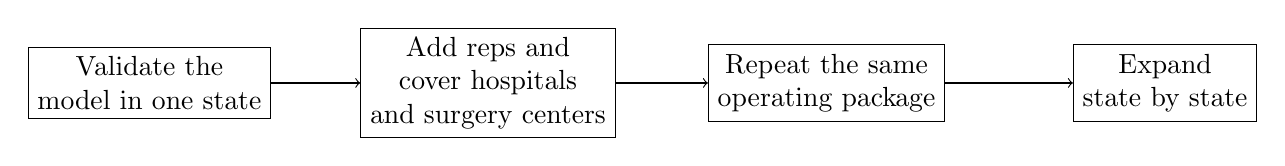
\begin{tikzpicture}
\node[draw, rectangle, align=center] (a) at (0,0) {Validate the\\model in one state};
\node[draw, rectangle, align=center] (b) at (4.3,0) {Add reps and\\cover hospitals\\and surgery centers};
\node[draw, rectangle, align=center] (c) at (8.6,0) {Repeat the same\\operating package};
\node[draw, rectangle, align=center] (d) at (12.9,0) {Expand\\state by state};
\draw[->] (a) -- (b);
\draw[->] (b) -- (c);
\draw[->] (c) -- (d);
\end{tikzpicture}
\caption{Editorial reconstruction of the lecture's turnkey scaling logic.}
\end{figure}

This is the point at which the lecture sounds most like a set of notes on business mechanics. We do not scale by cheering ourselves into growth. We scale by proving one unit of operation and then carrying that unit into neighboring terrain.

\subsection{Question \& Answer}

\paragraph{Question.} How can growth itself almost kill a company?

\paragraph{Answer.} Because growth is not merely a rise in revenue. It is also a rise in backlog, production pressure, and working-capital demand. When demand outruns capacity, success can become the mechanism of distress.

A compact update model makes the logic explicit:
\begin{align}
B_{t+1} &= B_t + Q_t - C_t,\\
K_{t+1}^{\mathrm{req}} &= k\,B_{t+1}.
\end{align}
Here $Q_t$ is incoming demand, $C_t$ is productive capacity, $B_t$ is backlog, and $k$ is the working capital required per unresolved unit.

The lecture's logic then unfolds in short steps.
\begin{enumerate}
\item If $Q_t > C_t$, then backlog rises.
\item If backlog rises, required working capital rises with it.
\item If available liquidity does not rise fast enough, the firm becomes constrained by its own success.
\end{enumerate}
In schematic form,
\begin{equation}
g_{\mathrm{sales}} > g_{\mathrm{capacity}}
\;\land\;
K_t < K_t^{\mathrm{req}}
\;\Rightarrow\;
\text{growth distress}.
\end{equation}

This is the meaning of the line that more companies die from indigestion than starvation. The company did not nearly die because customers disappeared. It nearly died because demand arrived faster than product and cash could be organized to meet it. The lecture is careful here. It does not withdraw the replication doctrine; it places a boundary on it. Growth must be sustainable, not merely rapid.

\section{Product Discovery, Market Pull, and the Sponsor Aside}

From the low point the lecture asks a better question: how does one find the winning product? The answer is cumulative and empirical. The entrepreneur says he had previously been a poor stockbroker. What changed was not a sudden flash of genius, but years of contact with doctors and surgery centers.

The sequence is worth preserving.
\begin{enumerate}
\item Stay close to the actual users and buyers.
\item Notice a problem that others are not attacking well.
\item Improve the product steadily, month by month, over years.
\item Reach a point at which demand begins to pull the product rather than having to be pushed onto the market.
\end{enumerate}

If we want a compact formal shorthand for the repeated refinement, we may write
\begin{equation}
P_{n+1} = P_n + \delta_n,
\end{equation}
where $P_n$ is the product at stage $n$ and $\delta_n$ is the correction learned from user feedback at that stage. This equation is editorial rather than spoken, but it accurately captures the lecture's month-by-month logic.

The lecture's payoff comes when sales calls stop feeling like pure persuasion. In the entrepreneur's description, the product becomes desirable enough that people hear about it, ask for it, and testify that it changes outcomes. The narrator then recaps the lesson in his own voice: years of back-and-forth with prospective clients exposed real problems, and solutions to those problems produced winning products that sold for millions.

\paragraph{Sponsor Aside.} At exactly this point the lecture is interrupted by a sponsor message about communication automation. Since it is structurally separate from the interview material, we preserve that separation in the notes. The numerical claims are
\begin{equation}
p_{\mathrm{auto}} \le 90\%, \qquad
p_{\mathrm{cost\,reduction}} \approx 30\%.
\end{equation}
These figures belong to the advertisement's rhetoric of leverage and efficiency. They are not part of the lecture's main chain of evidence about ownership, scale, or product discovery.

\section{Opportunity, Public Narratives, and Market Psychology}

After the sponsor, the lecture returns to the golf course and broadens in scope. The next older businessman restates the large exits---roughly \$25 million and \$200 million---and then, when asked what he would tell his younger self, begins not with a tactic but with a temporal warning: do not waste time.

From there the argument expands into a civic picture. In his telling, America remains a place of opportunity, especially for those who work without entitlement. He then gives a set of political-economy numbers, which we retain as interview claims rather than externally verified statistics:
\begin{equation}
p_{\mathrm{free\,enterprise}} \approx 87\%, \qquad
N_{\mathrm{billionaires}} \approx 750, \qquad
N_{\mathrm{population}} \approx 350\times 10^6.
\end{equation}
These numbers support his point that in a society committed to free enterprise, highly unequal commercial outcomes will occur. The lecture does not pause to prove those figures; it uses them rhetorically to defend the legitimacy of extreme success.

The same speaker then turns from statistics to analogy. On the golf range, he says, it would be absurd to ask that Tiger Woods be made less effective simply because he is too successful. The analogy is meant to expose a certain resentment toward excellence. Whether we agree with the politics or not, the lecture's motion is clear: it wants younger listeners to distrust shallow narratives and to study facts before forming opinions.

A final interview with a retired intellectual-property lawyer then narrows the frame again. He reports a peak earning year of about \$1 million and, when asked for the best financial advice he received, gives the standard Buffett line: be greedy when others are scared, and scared when others are greedy.

\subsection{Question \& Answer}

\paragraph{Question.} If everyone knows ``buy low, sell high,'' why do so many people act the other way around?

\paragraph{Answer.} Because crowd emotion reverses the timing of action. Rising prices make people want in; falling prices make people want out. The difficulty is not the algebra of the slogan but the psychology of acting against the crowd.

In minimal notation, the desired trading relation is
\begin{equation}
P_{\mathrm{buy}} < P_{\mathrm{sell}}.
\end{equation}
But the lecture insists that sentiment often pushes in the opposite direction:
\begin{align}
\sigma_{\mathrm{fear}} &\Rightarrow \text{accumulate},\\
\sigma_{\mathrm{greed}} &\Rightarrow \text{de-risk}.
\end{align}
The point is not that one can mechanically time every market. The point is that successful judgment often requires resisting the emotional motion of the crowd.

The lawyer's closing answers give the lecture a more human coda. When asked what he would tell his younger self, he says: if you are going through hell, keep going. He then speaks of faith, coincidence, and the experience that low periods do not last forever. Finally, when asked to choose between book smarts and street smarts, he answers in favor of the latter and underscores the point with the rhetorical question, How many differential equations does one solve in the real world? We should hear that carefully. The lecture is not repudiating thought. It is insisting that commercial life requires timing, reading of situations, and practical judgment in addition to formal learning.

\section{Summary}

The lecture opens with big numbers, but its durable content is not numerical spectacle. It is structural. Wealth is tied to ownership; ownership must be financed on the right time scale; scale comes from proving a model and repeating it; rapid growth can become destructive when capacity and cash lag demand; good products are discovered through long contact with real users; and markets reward those who can think against the emotional movement of the crowd.

By the end, the lecture has widened from business mechanics to public philosophy. It asks us to think carefully about opportunity, to distrust shallow resentment and shallow optimism alike, and to see that judgment is always doing two things at once: reading the structure of the business and reading the psychology of the world around it. That is why the lecture feels coherent despite its shifting locations. The golf course, the mansion, the sponsor interruption, and the late reflections on free enterprise all turn on the same question: what kind of disciplined ownership, thought, and timing actually produce durable wealth?